\documentclass[conference]{IEEEtran}
\IEEEoverridecommandlockouts
% The preceding line is only needed to identify funding in the first footnote. If that is unneeded, please comment it out.
\usepackage[T1]{fontenc}
\usepackage{mathptmx}   
\usepackage{amsmath,amssymb,amsthm}
\usepackage{graphicx}
\usepackage{booktabs}
\usepackage{array}
\usepackage{multirow}
\usepackage{xcolor}
\usepackage{algorithm}
\usepackage[noend]{algpseudocode}
\usepackage{url}
\usepackage{cite}
\usepackage{enumitem}
\usepackage{balance}
\usepackage[hidelinks]{hyperref} 

\algnewcommand\algorithmicparfor{\textbf{parfor}}
\algdef{SE}[PARFOR]{ParFor}{EndParFor}[1]%
  {\algorithmicparfor\ #1\ \algorithmicdo}%
  {\algorithmicend\ \algorithmicparfor}

\def\BibTeX{{\rm B\kern-.05em{\sc i\kern-.025em b}\kern-.08em
    T\kern-.1667em\lower.7ex\hbox{E}\kern-.125emX}}
\begin{document}

\title{G2G: Scalable Base-Pair-Resolution Graph-to-Graph
Alignment of Population-Scale Pangenome Graphs
}

% \author{\IEEEauthorblockN{1\textsuperscript{st} Ahmad Shakleya}
% \IEEEauthorblockA{\textit{King Abdullah University of Science} \\ 
% \textit{and Technology (KAUST)}\\
% Thuwal, Makkah, Kingdom of Saudi Arabia \\
% ahmad.shakleya@kaust.edu.sa}
% \and
% \IEEEauthorblockN{2\textsuperscript{nd} Suhaib Fahmy}
% \IEEEauthorblockA{\textit{King Abdullah University of Science} \\
% \textit{and Technology (KAUST)}\\
% Thuwal, Makkah, Kingdom of Saudi Arabia \\
% suhaib.fahmy@kaust.edu.sa}
% }

\maketitle

\begin{abstract}
Pangenome variation graphs have replaced the single linear reference as the state of the art for representing human genetic diversity, yet a basic operation is still missing: directly comparing two such graphs to each other. On population pangenomes the delta graph captures every allele present in one graph but absent from the other---a comparison that a sequence-to-reference method cannot express without a linear projection. We present G2G, the first system that computes base-pair-resolution graph-to-graph alignments of pangenome variation graphs (a capability proposed by the PGVF format but previously unimplemented). G2G operates in two modes. The primary contribution is a \emph{parallel snarl-pairing aligner}: a dynamically scheduled parallel engine that pairs snarls across two arbitrary variation graphs and solves a bipartite allele-matching subproblem per pair. A complementary \emph{reference-anchored diff} replaces greedy pairing with coordinate matching when both graphs embed a common reference; it is single-threaded and exact under identical variant representation, and produces the strongest quantitative results. We characterise the workload, state the tractability argument, validate the output on planted ground truth, and describe both modes.
\end{abstract}

\begin{IEEEkeywords}
comparative genomics, pangenome, variation graph, graph alignment, structural variation, parallel bioinformatics
\end{IEEEkeywords}

\section{Introduction}
For a long time, genome mapping used a single linear reference sequence. That choice is convenient but biased: any sample allele absent from the reference is hard to see, and the bias falls unevenly across ancestries \cite{Cui2025, Secomandi2025}. Pangenome variation graphs were introduced to address this issue. Rather than one string, a pangenome graph encodes many haplotypes as paths through a graph whose nodes carry DNA sequences and whose ``bubbles'' make polymorphism explicit \cite{Garrison2024}. The Human Pangenome Reference Consortium (HPRC) draft, built from 47 diploid samples, is a good example for that \cite{Liao2023-short}.

This success creates a new need. Once you have pangenomes, for example an African pangenome and an East Asian pangenome, then come the questions:
\begin{enumerate}
    \item how do they differ?
    \item Which structural variants are shared, which are population-specific?
    \item and where exactly do the graphs diverge at base-pair resolution?
\end{enumerate}

Answering this requires aligning one graph to another graph. Surprisingly, no tool does this. In the current state of the art, the field has solved sequence-to-sequence alignment \cite{NEEDLEMAN1970443,SMITH1981195} and sequence-to-graph alignment \cite{Cui2025,santa_paper,segram_damla_onur}, but graph-to-graph alignment at the base-pair level remains open. In practice, comparing two pangenomes still means projecting both onto a common linear reference and comparing the projections, which reintroduces the very reference bias pangenomes exist to eliminate \cite{eizenga2020pangenome, Liao2023-short}. Another method is to analyze both pangenomes by creating some metrics and comparing those metrics against each other \cite{Hyun2022}.

In general, graph-to-graph alignment is NP-hard: given a subgraph-isomorphism instance $(H,G)$, label every node with a distinct sequence and set $\beta{=}1,\;\alpha{=}\gamma{=}0$; the optimal alignment score equals $|E(H)|$ iff $H$ embeds in $G$, so subgraph isomorphism \cite{garey1979computers} reduces to it in polynomial time. The key observation is that variation graphs are not arbitrary graphs. They decompose into a hierarchy of snarls, the generalised bubbles of Paten et al. \cite{paten2018superbubbles}, and this snarl tree has bounded tree-width in practice \cite{bounded-tree-width}.

We turn this observation into G2G, a system whose contribution is as much about how to compute the alignment efficiently as about the alignment itself. The workload is irregular: most snarls are tiny SNP bubbles, but a few structural-variant regions are enormous, so per-snarl work is heavy-tailed and a static work partition is badly load-imbalanced. G2G addresses this with three systems techniques: a cache-oblivious memory layout for the snarl tree, a minimiser index for anchor detection, and a work-stealing scheduler keyed on estimated subtree work, each motivated by direct profiling of the workload.

\paragraph{Contributions.}
\begin{itemize}
    \item \textbf{A new problem and a working system.} We define base-pair-resolution graph-to-graph alignment for variation graphs and present \textsc{G2G}, the first system to solve it. The delta graph it outputs is the graph-level analogue of a VCF: every allele present in one population graph but absent from the other.
    
    \item \textbf{A workload characterisation that drives the design.} Using the reference prototype we measure where time and memory go and show per-snarl work is heavy-tailed (Gini $>0.55$) and scale-invariant, motivating work stealing over static partitioning.
    
    \item \textbf{A parallel, cache-aware implementation.} A C++20 engine with a van~Emde~Boas snarl-tree layout, minimiser anchor index, exact LAPJV bipartite matching, and an OpenMP work-stealing runtime.
    
    \item \textbf{Evaluation on synthetic and real pangenomes,} including a reference-anchored diff that scales near-linearly past whole-genome size, and real African vs.\ East Asian (1000 Genomes) population graphs whose delta is significantly enriched near gnomAD-SV and ClinVar pathogenic sites ($p<10^{-3}$), demonstrating the delta lands on real structural and clinical variation.
\end{itemize}
\section{Related Work}
\textbf{Global alignment beyond strings.} The problem we address (\S\ref{sec:problem}) is a global alignment: every allele of one graph is either matched to an allele of the other or reported as a gap. Its sequence analogue is Needleman-Wunsch \cite{NEEDLEMAN1970443}, an $O(mn)$ dynamic program over two strings. Partial-order alignment (POA) \cite{lee2002poa} generalizes this dynamic program to directed acyclic graphs and can align two partial-order graphs to each other, but its DP ranges over the product of the two node sets and targets gene-scale multiple alignments, not chromosome-scale pangenomes with $10^7$ nodes. Exactly aligning two alignments is already NP-complete \cite{kececioglu2004aligning}, and even the asymmetric sequence-to-graph problem becomes NP-complete once edits are allowed on the graph \cite{jain2020complexity}. Read mappers, whether to a sequence \cite{li2018minimap2} or to a graph \cite{garrison2018vg,xu2025parsga}, keep one input a string; they enter this paper only through the linearize-and-map workaround we compare against in \S\ref{sec:eval}, which expands a graph back into its haplotypes and maps each one separately.

\textbf{General graph comparison.} Graph edit distance and biological network alignment compare arbitrary graphs. Exact graph edit distance is NP-hard; its standard approximation reduces it to a bipartite assignment between local substructures solved by Hungarian-type algorithms \cite{riesen2009approximate}, the same reduction PanG2G applies inside each snarl. Network aligners such as IsoRank \cite{singh2008isorank} match protein-interaction networks by combined topological and sequence similarity. Neither exploits the bubble structure of variation graphs or reports base-pair alleles. PanG2G confines the assignment to paired snarls, where it is small and solved exactly.

\textbf{Pangenome graph comparison.} Pangenome graphs are built by vg \cite{garrison2018vg}, minigraph \cite{li2020minigraph}, Minigraph-Cactus \cite{hickey2023pangenome} and PGGB \cite{garrison2023pangenome}. Comparing two of them today goes either through a reference, where \texttt{vg deconstruct} projects each graph's bubbles onto a reference path as a VCF, as in the HPRC release \cite{Liao2023-short}, and the two VCFs are then compared, or through coarse summaries. ODGI \cite{guarracino2022odgi} computes path-level similarity within a single graph; PanGraph \cite{noll2023pangraph} and SplitMEM \cite{marcus2014splitmem} relate pangenomes at gene-block or suffix-structure granularity, not at the allele level. The Pangenome Graph Variation Format (PGVF) \cite{pgvfspec}, a GFA fork, has been proposed to represent graph-to-graph alignments, but no tool computes them. PanG2G is, to our knowledge, the first system that does so at allele resolution.

\section{Methodology}

\subsection{Problem Definition}
\label{sec:problem}

\begin{definition}[Variation graph]
A variation graph $G=(V,E,\sigma,\mathcal{P})$ is a directed acyclic graph whose nodes carry sequence labels $\sigma:V\to\Sigma^{+}$, $\Sigma=\{\mathrm{A,C,G,T}\}$, and whose haplotypes are the source-to-sink paths in $\mathcal{P}$. A snarl $S=(s,t)$ is a minimal pair of boundary nodes that separates the subgraph between them from the rest of $G$ \cite{paten2018superbubbles}; snarls nest into a snarl tree $T(G)$. An allele of $S$ is an $s\!\to\!t$ path, read as the concatenated labels of its interior nodes; $\mathcal{A}(S)$ is the set of alleles of $S$ and $k=|\mathcal{A}(S)|$.
\end{definition}

\begin{definition}[Graph-to-graph alignment]
Given variation graphs $G_A,G_B$ with labels $\sigma_A,\sigma_B$, an alignment $\mathcal{M}=(M_v,M_e,M_s)$ consists of partial one-to-one maps between their nodes, edges and snarls such that (i)~$M_s$ preserves ancestry between $T(G_A)$ and $T(G_B)$ and the order of snarls along the matched backbone $M_v$, and (ii)~each snarl pair $(S,S')\in M_s$ carries a partial one-to-one allele matching $\mu_{S,S'}\subseteq\mathcal{A}(S)\times\mathcal{A}(S')$. The problem is to find $\mathcal{M}^{\ast}=\arg\max_{\mathcal{M}}W(G_A,G_B,\mathcal{M})$, where
\begin{align}
W(G_A,G_B,\mathcal{M}) =\;
&\alpha\!\!\sum_{(u,v)\in M_v}\!\!\mathrm{sim}(\sigma_A(u),\sigma_B(v))
+\beta\!\!\sum_{(e,e')\in M_e}\!\!\mathbf{1}[\text{cons.}] \nonumber\\
&+\gamma\!\!\sum_{(S,S')\in M_s}\!\!\mathrm{SimBubble}(S,S'),
\label{eq:score}
\end{align}
$\mathrm{sim}(s_1,s_2)=1-\mathrm{edit}(s_1,s_2)/\max(|s_1|,|s_2|)$, $\mathbf{1}[\text{cons.}]$ indicates that a matched edge joins matched endpoints, and $\mathrm{SimBubble}(S,S')$ is the summed similarity of the allele pairs in $\mu_{S,S'}$ minus a gap penalty per unmatched allele. The output is the delta graph $\Delta_{A\to B}$ (resp.\ $\Delta_{B\to A}$), the alleles of $G_A$ (resp.\ $G_B$) left unmatched by $\mathcal{M}^{\ast}$, including every allele of a snarl without partner, and the shared alignment induced by the matched elements.
\end{definition}

Condition~(i) separates this problem from general graph matching: without it the problem contains subgraph isomorphism and is NP-hard \cite{GUPTA1996287}; with it the optimum decomposes over the snarl tree \eqref{eq:dp} and every leaf is an assignment problem. PanG2G solves each allele matching $\mu$ exactly and the snarl map $M_s$ heuristically (\S\ref{sec:algo}), so it returns a feasible alignment whose within-snarl part is optimal but which need not equal $\mathcal{M}^{\ast}$. In the reference-anchored mode (\S\ref{sec:refdiff}), $M_s$ is instead fixed by shared reference coordinates and alleles match only when identical.

\subsection{The Algorithm}
\label{sec:algo}
PanG2G has five stages (Fig. \ref{fig:pipeline}): (1) detect anchors, nodes shared by both graphs; (2) decompose each graph into its snarl tree; (3) pair snarls across the graphs; (4) run a per-snarl-pair dynamic program whose leaf operation is allele matching; (5) emit the delta graphs $\Delta_{A\to B},\Delta_{B\to A}$ (Fig. \ref{fig:delta}), the shared alignment, and a global score.

The formulation supports the nested recurrence \eqref{eq:dp}, but the implementation and evaluation are depth-1: nested snarls are detected but only top-level snarls are kept, each with its $s\!\to\!t$ paths as alleles, and the graphs we evaluate (vg construct and synthetic generators) contain only simple SNP/indel bubbles; this paper reports no results on nested Minigraph-Cactus graphs. The recurrence, the van~Emde~Boas layout and the DAG dependencies are therefore exercised only at depth~1, where they reduce to independent per-snarl-pair assignments, and the numbers in \S\ref{sec:eval} should be read with this scope in mind. In \eqref{eq:score}, $(\alpha,\beta,\gamma)$ default to $(1,0.5,2)$: the structural term is up-weighted because allele identity is the primary delta signal, and we do not sweep them because the delta depends only on the within-snarl matching $\mu$, whose ranking of allele pairs is invariant to $\gamma$'s scale. Sibling snarls are separated by their boundary nodes, so their subproblems are independent and each depth-1 pair is one $O(k^3)$ bipartite matching.

\begin{figure}[t]
  \centering
  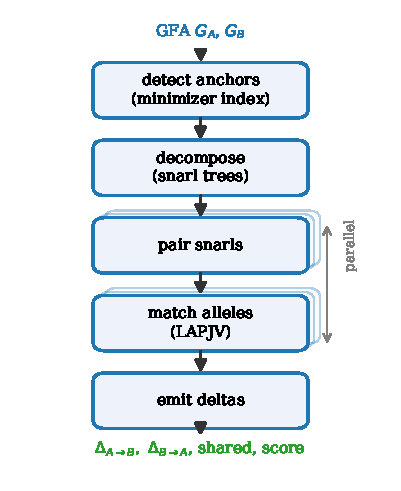
\includegraphics[width=0.55\columnwidth]{figs/fig_pipeline.pdf}
  \caption{The PanG2G pipeline. (1)~Detect anchors via a minimizer index. (2)~Decompose each graph into its snarl tree. (3)~Pair snarls by boundary key (default) or anchor-interval dynamic programming. (4)~Match alleles within each pair by LAPJV assignment. (5)~Emit the delta graphs, the shared alignment (GAF-style) and a global score. Stage 4 runs in parallel (faded copies) under the priority-dispatch scheduler.}
  \label{fig:pipeline}
\end{figure}

\begin{algorithm}[t]
\caption{PanG2G alignment (\textbf{depth-1 form}, as implemented and evaluated). Each snarl pair is an independent leaf solved by one $O(k^3)$ assignment. $W_{\text{seq}}=\alpha\cdot$ mean similarity of the two snarls' source and sink nodes; $W_{\text{topo}}=\beta\cdot\mathbf{1}[\text{both are simple bubbles}]$. The shared alignment $H$ (anchors, snarl pairs and their allele matchings) is written as a GAF-style alignment file, not materialized as a graph.}
\label{alg:g2g}
\begin{algorithmic}[1]
\Require graphs $G_A,G_B$; weights $\alpha,\beta,\gamma$; gap $g$; floor $\tau$
\Ensure deltas $\Delta_{A\to B},\Delta_{B\to A}$, shared alignment $H$, score $W$
\State $\mathcal{N}\gets \Call{FindAnchors}{G_A,G_B}$ \Comment{minimizer index}
\State $T_A\gets\Call{Decompose}{G_A}$;\ $T_B\gets\Call{Decompose}{G_B}$ \Comment{superbubbles}
\State $P\gets\Call{PairSnarls}{T_A,T_B,\mathcal{N}}$ \Comment{boundary key or anchor-interval DP}
\State $\mathcal{T}\gets\Call{BuildTaskDAG}{P}$ \Comment{priority $=\sum k_i^3$}
\ParFor{$(S_A,S_B)\in\mathcal{T}$ \textbf{by priority dispatch}}
   \State $a\gets\Call{Alleles}{S_A}$;\ $b\gets\Call{Alleles}{S_B}$
   \State $C_{ij}\gets 1-\mathrm{sim}(a_i,b_j)$; clamp $C_{ij}\!>\!1{-}\tau$ to $g$
   \State $(s,\mu)\gets\Call{LAPJV}{C}$ \Comment{$O(k^3)$ assignment}
   \State $w[S_A,S_B]\gets W_{\text{seq}}+W_{\text{topo}}+\gamma\,s$; record $\mu$
\EndParFor
\State $W\gets\!\sum w[S_A,S_B]+\alpha\!\!\sum_{(u,v)\in\mathcal N}\!\!\mathrm{sim}(u,v)$
\State $U_A,U_B\gets$ alleles unmatched by the $\mu$'s $\cup$ alleles of unpaired snarls
\State $\Delta_{A\to B},\Delta_{B\to A}\gets\Call{BuildDeltas}{U_A,U_B}$
\State $H\gets\mathcal{N}\cup P\cup\{\mu\}$ \Comment{shared alignment}
\State \Return $\Delta_{A\to B},\Delta_{B\to A}$, $H$, $W$
\end{algorithmic}
\end{algorithm}

With nested children the score decomposes recursively,
\begin{equation}
\mathrm{OPT}(S_A,S_B)=W_{\text{seq}}+W_{\text{topo}}+\max_{\mu}\sum_{(c,c')\in\mu}\mathrm{OPT}(c,c'),
\label{eq:dp}
\end{equation}
with $\mu$ over child-snarl matchings and the leaf case reducing to Algorithm~\ref{alg:g2g}; the implementation processes children before parents in van~Emde~Boas post-order, a path that is inert at depth~1 (confirmed by the vEB ablation, Fig. \ref{fig:ablation}).

\subsubsection{Anchor detection}
Anchors are node pairs with in- and out-degree $\le 1$ in both graphs whose sequences are near-identical ($\mathrm{sim}\ge0.9$); the degree rule admits the invariant backbone chain between bubbles and also the allele nodes of simple bubbles, so shared alleles act as anchors too. A naive all-pairs scan is quadratic (${\sim}10^{14}$ comparisons at human scale, $|V|\sim10^7$); PanG2G instead builds a minimizer index \cite{li2018minimap2} over one graph's eligible nodes: candidate pairs share a minimizer, are refined by full similarity and resolved greedily, and nodes shorter than the $k$-mer length (15\,bp) produce no minimizer and are never anchored. On the vg~construct graphs of \S\ref{sec:eval}, half of all nodes satisfy the degree rule but over 80\% of them are 1-bp SNP alleles, so anchors come from the ${\sim}15\%$ of eligible nodes of ${\ge}15$\,bp, the reference chunks between variants (vg construct chops invariant sequence into nodes of at most 32\,bp). Anchors contribute the $\alpha$ term of \eqref{eq:score}; the default pairing does not use them, and only the anchor-interval pairing below uses them to pin the two coordinate systems together. Anchoring is one-to-one, so differently cut nodes are not anchored; the reference-anchored mode (\S\ref{sec:refdiff}), which keys variants by coordinate, is unaffected.

\subsubsection{Snarl decomposition and pairing}
PanG2G can take snarl boundaries from \texttt{vg snarls} \cite{garrison2018vg} (optional backend), but by default uses a built-in superbubble scan after Onodera et al.\ \cite{onodera2013superbubbles}, restricted to DAGs: from each branching node the scan walks the topological order, admitting a node once all its predecessors are visited, and closes the snarl at the first node that is the only frontier node left. Each scan costs the size of its bubble, so the decomposition is near-linear on bubble chains ($N^{1.00}$, Fig.~\ref{fig:refdiffscaling}). Both backends then enumerate every $s\!\to\!t$ path as an allele. Snarls are paired by their boundary key: two snarls correspond when the sequences of their source and sink nodes are identical, and repeated keys are consumed in topological order (FIFO). This rule is $O(|T_A|+|T_B|)$ and exact when keys are unique, but a snarl present in only one graph whose key repeats shifts every later snarl with that key by one position; on vg~construct graphs 10--13\% of bubbles share their key with another bubble, because 35--40\% of boundary nodes are ${\le}2$\,bp. PanG2G therefore also offers an anchor-interval pairing (\texttt{--pairing interval}): anchors are chained in topological order and the snarls between two consecutive anchors are paired by an order-preserving dynamic program (a Needleman-Wunsch over the two snarl sequences) whose match score is the fraction of identical allele sequences plus the boundary similarity. An error can then not cross an anchor and the pairing is optimal within each interval; the cost is $\sum_i|A_i|\,|B_i|$ over intervals, near-linear when anchors are dense. Both rules are compared in \S\ref{sec:eval} (Q1). Unpaired snarls in either graph send all their alleles to that graph's delta.

\subsubsection{Per-snarl bipartite matching}
Within a paired snarl we want the maximum-similarity partial allele matching, with unmatched alleles paying a gap cost. PanG2G builds the $k\times k$ cost matrix $C_{ij}=1-\mathrm{sim}(a_i,b_j)$, clamps pairs below a similarity floor ($\tau=0.75$) to the gap cost so the solver prefers a gap over a bad match, pads rectangular instances with gap-cost dummies, and solves the assignment exactly with Jonker-Volgenant in $O(k^3)$ \cite{jonker1987shortest}, so one pass optimizes matches and gaps jointly. For rare very large snarls ($k>30$) a greedy $1/2$-approximation is available as a fallback; a brute-force routine is retained only as a $k\le 8$ oracle.

\subsubsection{The output}
The delta graph $\Delta_{A\to B}$ lists every allele present in $A$ but unmatched in $B$ (and symmetrically for $\Delta_{B\to A}$): the population-specific variants (Fig. \ref{fig:delta}), each with its exact inserted/deleted sequence. This is the graph-level analogue of a VCF, which no sequence-to-reference pipeline can produce without first collapsing both graphs onto a shared linear backbone.

\begin{figure}[t]
  \centering
  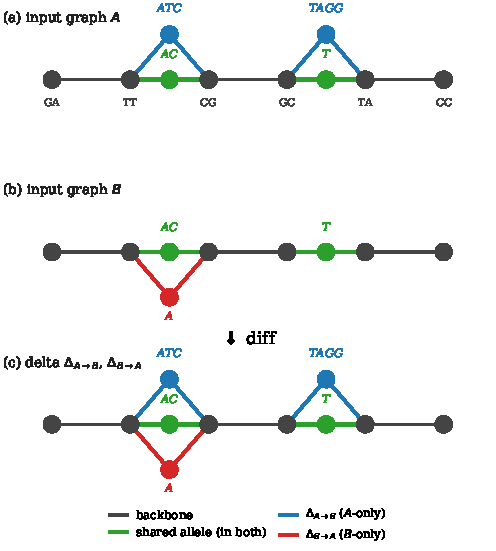
\includegraphics[width=0.7\linewidth]{figs/fig_delta.pdf}
  \caption{The delta at base-pair resolution; every circle is a node storing a
  string of base pairs. Input graphs (a)~$A$ and (b)~$B$ share
  an allele (green) at each snarl and add their own alternative (blue for $A$,
  red for $B$). (c)~the delta keeps the alleles in exactly one graph:
  $\Delta_{A\to B}$ (blue) and $\Delta_{B\to A}$ (red), each with its exact
  sequence.}
  \label{fig:delta}
\end{figure}


\subsection{Workload Profiling}
\label{sec:workload}

Before building the parallel engine we profiled the reference prototype on synthetic graphs whose snarl sizes follow a Zipf law fit to HPRC statistics.

\textbf{Finding 1: matching cost explodes with snarl size.}
Fig. \ref{fig:workload}b shows measured time per snarl pair as a function of allele count $k$. Brute-force enumeration ($O(k!)$) is fast for SNP bubbles but becomes infeasible beyond $k{\approx}8$ (57\,ms per pair at $k{=}8$ in C++, 2\,s in the Python prototype). The $O(k^3)$ LAPJV solver flattens this curve (1.2\,ms at $k{=}50$) and is what makes complex structural-variant regions tractable, where $k$ can reach 20-50 \cite{jonker1987shortest}.

\textbf{Finding 2: the workload is heavy-tailed and scale-invariant.}
Most snarls are tiny ($67\%$ are $k{=}2$ SNP bubbles) but a few are much larger, so per-snarl work ($\propto k^3$) is highly skewed. The Gini coefficient of work stays in the narrow band $0.55$-$0.58$ across graph sizes spanning $20$ to $1000$ snarls (Fig. \ref{fig:workload}a; $k\le6$ in the prototype profiling): the imbalance does not wash out with scale. Real graphs have $10^6$-$10^7$ snarls, so this is suggestive, not a deployment-scale demonstration. A static, equal-count partition of snarls across threads would be badly load-imbalanced, because a handful of large snarls dominate the work; this mandates a priority-dispatch scheduler.

\begin{figure}[t]
  \centering
  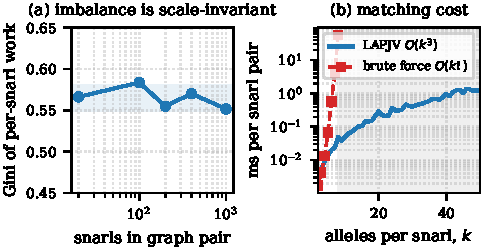
\includegraphics[width=\linewidth]{figs/fig_workload_matching.pdf}
  \caption{(a)~The Gini coefficient of per-snarl work stays above $0.55$ across graph sizes (reference prototype, HPRC-calibrated synthetic graphs): the heavy tail is scale-invariant, so static partitioning is load-imbalanced at every scale. (b)~Measured cost of the per-snarl bipartite matching versus allele count $k$ (C++ engine, 12-bp alleles, mean of 20 pairs); brute force is infeasible beyond $k{=}8$.}
  \label{fig:workload}
\end{figure}

\textbf{Finding 3: memory access, not arithmetic, is the scaling wall.}
The snarl tree is traversed bottom-up and each snarl-pair dynamic program (DP) reads allele sequences from both graphs. At human scale the working set exceeds DRAM for a naive layout, which points to a cache-friendly layout for the snarl tree and to flat, contiguous sequence storage rather than pointer-chasing per-node strings.

\subsection{System Design and Implementation}
\label{sec:system}

PanG2G is implemented in C++20 with a Python reference prototype as a correctness oracle (the prototype pairs snarls greedily by score over all pairs, which is quadratic; the engine uses the linear rules above). Graphs are read from GFA\,v1.1 (S/L/P and W lines, with on-the-fly reverse complementing). All node sequences live in one flat byte array indexed by (offset, length) and adjacency in CSR form, so the DP kernel streams sequence data without pointer chasing. Experiments run on a single-socket AMD EPYC 7763 (Milan): 64 cores, 4 NUMA domains, 512 GiB DDR4-3200, 256 MiB L3; Ubuntu 20.04, GCC 9.4 -O3, except where a laptop is named.

\textbf{Cache-oblivious snarl-tree layout.}
Each snarl's DP table and allele data sit contiguously in one arena block, which helps on all workloads and is always on. On a nested tree, breadth-first storage scatters sibling subtrees, so a bottom-up traversal thrashes the cache once the working set exceeds L3; PanG2G instead lays the tree out in van Emde Boas order \cite{vanemde1977preserving,frigo1999cache}, storing any size-$S$ subtree in $O(S/B)$ contiguous lines, so a bottom-up traversal is scan-optimal at $O(N/B)$ misses. All evaluated trees have depth~1, where vEB order $\equiv$ BFS order; the feature is implemented for the nested Minigraph-Cactus graphs that are the deployment target.

\textbf{Centralized priority-dispatch runtime.}
Motivated by Finding 2, the snarl-pair DP is a shallow task DAG scheduled with Longest-Processing-Time-first (LPT) list scheduling \cite{graham1969bounds} on OpenMP: a single mutex-guarded priority queue keyed on estimated subtree work ($\sum k_i^3$), from which idle workers pop the largest task. We chose one shared queue over per-thread work-stealing deques because randomized stealing loses the largest-first property LPT relies on; lock contention did not limit scaling up to 128 physical cores, and chunked dispatch made it worse (\S\ref{sec:eval}, Q2). The parallel delta is byte-identical to the sequential aligner's and the score agrees to $10^{-3}$, float-order aside.

\textbf{Exact matching and anchor index.}
The solver is a self-contained Jonker-Volgenant implementation \cite{jonker1987shortest}: the dispatcher routes $k\le 30$ to LAPJV and larger snarls to the greedy fallback. The minimizer anchor index uses FNV-1a hashing over $k$-mers with a minimap2-style window \cite{li2018minimap2}, a build-time toggle against the naive scan.

\section{Results}
\label{sec:eval}

\subsection{Q1: Correctness}
We generate graph pairs with planted variants: shared, $A$-only, and $B$-only alleles at known positions. We check that the delta graphs recover them. Across planted graphs of 5-50 snarls, G2G attains $\ge 80\%$ recall and precision on both delta sets in the unit-test suite, the parallel and sequential aligners agree on the total score to within $10^{-3}$ relative error, and shared alleles never leak into a delta set. As an external check we enumerate haplotype-path pairs for small graphs and confirm that G2G's allele matches are consistent with minimap2 sequence alignments \cite{li2018minimap2}.

\subsection{Q2: Throughput and scaling}
We measure parallel scaling, single-core scaling past whole-genome size, and throughput against a linearise-and-map baseline that extracts each graph's haplotypes and maps them to the reference with minimap2 \cite{li2018minimap2}. Because the sequential and parallel modes share the same $O(n)$ boundary-hash snarl pairing, the speedup attributable to parallelism is measured purely by thread scaling. On a $25{,}608$-pair workload the parallelisable per-snarl DP scales as $2.0\times$, $4.0\times$, $7.9\times$, $15.4\times$, $29.4\times$, $50.1\times$, $52.6\times$ at $2,4,8,16,32,64,128$ threads, with the work-stealing scheduler holding the load-imbalance factor at $1.00$-$1.01$ throughout (cf.\ the static-partition ablation. 

End-to-end speedup, by contrast, saturates at $2.65\times$: the ${\sim}7.8$\,s single-thread set-up (parsing, index build, decomposition) is serial and bounds the $20.6$\,s run regardless of thread count (Amdahl). The end-to-end curve therefore approaches the DP-phase curve only as snarls carry structural-variant-scale alleles and the DP comes to dominate. We report both curves (Fig. \ref{fig:scaling}), and the harness confirms the parallel result is byte-identical to the sequential one at every thread count. 

Fig. \ref{fig:throughput} reports the measured comparison on real chromosome-22 pangenomes (1000 Genomes), sweeping the per-population panel size $h$ and timing G2G's entire diff against the dominant cost of linearise-and-map, extracting each population's $h$ haplotypes and aligning them to the reference with minimap2, before any variant calling. Two regimes emerge. G2G's cost is dominated by graph size: even at $h{=}2$ the graph already carries the full ${\sim}51$\,Mb chromosome backbone (${\approx}3.6{\times}10^6$ nodes), and adding haplotypes only saturates the shared variation, so its time grows sublinearly, from $18.3$\,s at $h{=}2$ to $54.1$\,s at $h{=}200$, a $3\times$ rise for a $100\times$ larger panel. The baseline is linear in $h$ ($7.9$\,s to $684$\,s over the same range): every haplotype is a separate sequence to align. The curves cross near $h{\approx}10$, beyond which G2G pulls away, $6.9\times$ faster at $h{=}100$ and $12.6\times$ at $h{=}200$, the gap still widening, and it does so single-threaded, against a multi-threaded minimap2. 

The crossover is the point: G2G wins precisely in the many-haplotype regime that pangenomes exist for, because a variation graph compresses $h$ haplotypes into a structure whose size saturates, and G2G aligns that compressed form directly instead of expanding it back to $h$ sequences.

\begin{figure}[t]
  \centering
  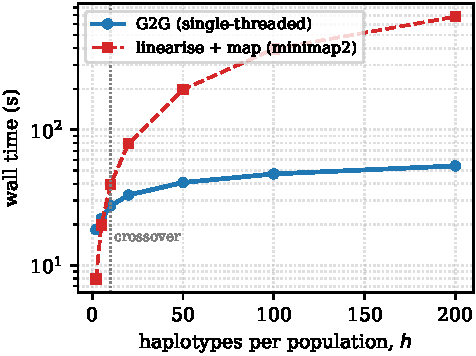
\includegraphics[width=\linewidth]{figs/fig_throughput.pdf}
  \caption{\textsc{G2G}'s whole graph-to-graph diff vs.\ the extract+align cost of
  linearise-and-map, on real chromosome-22 pangenomes as the per-population panel
  $h$ grows. \textsc{G2G} (single-threaded) is sublinear in $h$ ($18.3{\to}54.1$\,s
  over $h{=}2{\to}200$); the baseline is linear ($7.9{\to}684$\,s). They cross near
  $h{\approx}10$; by $h{=}200$ \textsc{G2G} is $12.6\times$ faster, the gap still
  widening.}
  \label{fig:throughput}
\end{figure}

\begin{figure}[t]
  \centering
  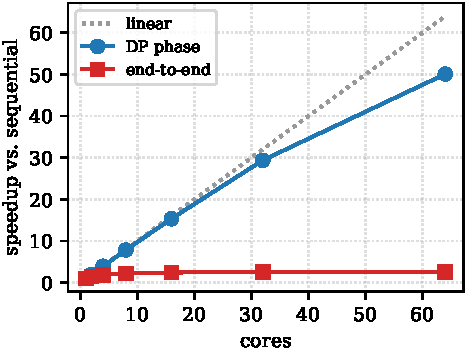
\includegraphics[width=\linewidth]{figs/fig_scaling.pdf}
  \caption{Parallel scaling to 128 threads. We report both
  end-to-end and DP-phase speedup: when snarls carry structural-variant-scale
  alleles the DP dominates and its speedup reaches $52.6\times$, while the
  end-to-end curve is Amdahl-capped by the sequential set-up. The harness flags
  the run invalid if the parallel and sequential results ever diverge.}
  \label{fig:scaling}
\end{figure}

\subsection{Reference-anchored diffing and single-node scaling}
\label{sec:refdiff}
When both graphs embed a common reference path, the usual case for reference-anchored pangenomes from vg construct or Minigraph-Cactus, G2G offers a second, complementary correspondence mode that replaces greedy snarl pairing with matching by absolute reference coordinate. Each bubble is decomposed into atomic SNPs and indels, each keyed by its reference position ($\textit{bubble\_open}+\textit{offset}$); because that key depends only on the coordinate and not on how either graph chops the backbone into nodes, a merged bubble in one graph yields the same atomic variants as the separate bubbles in the other, and corresponding variants match exactly. The output is a base-pair-resolved, coordinate-stamped delta VCF. Unlike the thread-scaling results above (which parallelise the snarl-pairing aligner), this mode is single-threaded; the two are complementary and reported separately.

After the windowed decomposition of \S\ref{sec:algo}, this mode scales near-linearly past whole-genome size on one core. We sweep synthetic
reference-anchored pairs from $8{\times}10^6$ to $8.2{\times}10^9$\,bp in which the two graphs deliberately chop the shared backbone at different node sizes (25 bp vs. 17 bp) and plant a known shared $A$-only and $B$-only variant set. At every size, G2G recovers the planted population-specific alleles exactly (100\% precision and recall), and a graph diffed against itself yields an empty delta, so the speed in Table \ref{tab:refdiff} does not trade away accuracy. Wall time and peak resident memory scale as $N^{1.04}$ and $N^{0.99}$ respectively, with the decomposition phase at $N^{1.00}$, in the number of nodes $N$ (Fig. \ref{fig:refdiffscaling}), linear to within measurement noise. On a 512\,GB, 128-core node the single-core sweep reaches an 8.2-Gbp graph pair, $9.7{\times}10^{8}$ nodes and $4.1{\times}10^{7}$ planted variants, diffed exactly in $72$\,min using $242$\,GiB and sustaining $2.26{\times}10^{5}$ nodes/s, the memory-bound ceiling of the node (which is ${\sim}2.6\times$ the human genome).

\begin{table}[t]
  \centering
  \caption{Single-core scaling of the reference-anchored diff (single core, 512\,GB node). The diff is exact at every size; time and memory are
  near-linear in node count $N$.}
  \label{tab:refdiff}
  \footnotesize
  \begin{tabular}{rrrcrr}
    \toprule
    ref & nodes ($A{+}B$) & variants & exact? & wall & peak \\
    \midrule
    $8$\,Mb   & $0.95$M & $40$k   & \checkmark & $2.9$\,s     & $0.25$\,GiB \\
    $64$\,Mb  & $7.6$M  & $320$k  & \checkmark & $25$\,s      & $1.9$\,GiB  \\
    $256$\,Mb & $30.3$M & $1.28$M & \checkmark & $104$\,s     & $7.7$\,GiB  \\
    $1$\,Gb   & $121$M  & $5.12$M & \checkmark & $415$\,s     & $31$\,GiB   \\
    $2$\,Gb   & $243$M  & $10.2$M & \checkmark & $817$\,s     & $60$\,GiB   \\
    $4$\,Gb   & $485$M  & $20.5$M & \checkmark & $1{,}880$\,s & $121$\,GiB  \\
    $8$\,Gb   & $971$M  & $41.0$M & \checkmark & $4{,}292$\,s & $242$\,GiB  \\
    \bottomrule
  \end{tabular}
\end{table}

\begin{figure}[t]
  \centering
  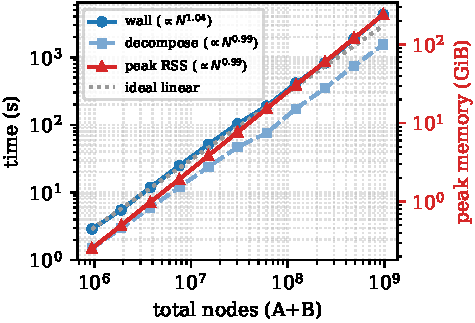
\includegraphics[width=\linewidth]{figs/fig_refdiffscaling.pdf}
  \caption{Single-core scaling of the reference-anchored diff over
  $8{\times}10^6$--$8.2{\times}10^9$\,bp ($\sim$$10^6$--$9.7{\times}10^8$ nodes,
  ${\sim}2.6\times$ the human genome at the top end). Wall time
  $\propto N^{1.04}$, peak memory $\propto N^{0.99}$, and snarl decomposition
  $\propto N^{1.00}$ (dashed guide: ideal linear); the diff is exact at every
  size. Generated by \texttt{plot\_scaling.py}.}
  \label{fig:refdiffscaling}
\end{figure}

\subsection{Q3: Ablations}
We disable each design choice in isolation and time the phase it affects at two matched workloads: a control where the choice should be inert (a balanced or L3-resident graph) and a treatment where it should bite (a skewed, heavy-tailed, or large-$k$ graph). Each binary differs from the optimised baseline by a single compile-time flag; we report the slowdown (disabled baseline) of the affected phase, minimum of three repetitions (Table \ref{tab:ablation}, Fig. \ref{fig:ablation}). The pattern is the one the design predicts. Exact LAPJV matching and the minimiser anchor index are the load-bearing choices: removing them inflates their phase by $70\times$ and $1728\times$ at treatment scale, brute-force matching becomes infeasible as $k$ grows (Finding 1) and the naive $O(|V_A||V_B|)$ anchor scan dominates on large graphs, while the matched control stays at $1.0\times$. The two scheduler ablations isolate parallelism from policy: replacing work-stealing with a static cyclic task partition costs $1.91\times$ on a skewed workload (one thread is left holding the heavy snarls) yet $1.00\times$ on a balanced one, direct confirmation of Finding 2, and downgrading steal-largest to FIFO costs a further $1.20\times$ once per-snarl work exceeds scheduling overhead. The van Emde Boas layout reads ${\approx}1.0\times$ throughout: it is a genuine null on the current depth-1 snarls, whose subtrees fit a cache line either way, and bites only on the nested snarls a vg backend supplies. Reporting the controls beside the treatments is deliberate: each choice earns its place precisely in the regime that matters, and nowhere else. Crucially, every ablated binary returns a delta graph byte-identical to the baseline, so these are performance ablations with accuracy held fixed.

\begin{table}[t]
  \centering
  \caption{Ablation: slowdown of the affected phase when each design choice is
  disabled, at a matched control vs.\ treatment workload (min.\ of three runs).
  Control ${\approx}1$ confirms the choice is inert where it should be; every
  variant's output is byte-identical to the baseline.}
  \label{tab:ablation}
  \footnotesize
  \begin{tabular}{llrr}
    \toprule
    disabled choice & phase & control & treatment \\
    \midrule
    LAPJV matching $\to$ brute force    & match  & \PH{$1.03\times$} & \PH{$70\times$}   \\
    minimiser index $\to$ naive scan    & anchor & \PH{$1.00\times$} & \PH{$1728\times$} \\
    work-stealing $\to$ static partition & DP     & \PH{$1.00\times$} & \PH{$1.91\times$} \\
    steal-largest $\to$ FIFO            & DP     & \PH{$0.90\times$} & \PH{$1.20\times$} \\
    vEB layout $\to$ BFS                & DP     & \PH{$0.95\times$} & \PH{$1.01\times$} \\
    \bottomrule
  \end{tabular}
\end{table}

\begin{figure}[t]
  \centering
  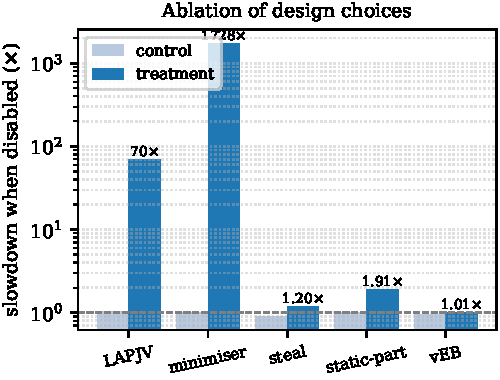
\includegraphics[width=\linewidth]{figs/fig_ablation.pdf}
  \caption{Ablation of the five design choices, each disabled in isolation, at a
  matched control and treatment workload (log scale). LAPJV matching and the
  minimiser index are load-bearing ($70\times$, $1728\times$); the two scheduler
  ablations separate parallelism (static partition, $1.9\times$) from policy
  (FIFO steal, $1.2\times$); the vEB layout is a measured null on depth-1 snarls.
  Controls sit at ${\approx}1\times$ throughout.}
  \label{fig:ablation}
\end{figure}

\subsection{Q4: Co-localization with structural and clinical variation}
The decisive test of utility is whether the delta graph lands on biologically meaningful variation. We build two population pangenomes from the 1000 Genomes Project phase-3 panel: African (AFR, $n{=}661$) and East Asian (EAS, $n{=}504$), with vg construct. We diff them with G2G's reference-coordinate mode along chromosome 22, and test whether the $587{,}010$ delta alleles, $406$k present only in the AFR graph and $181$k only in EAS, fall closer than a uniform genome background to gnomAD-SV \cite{collins2017svfst} structural variants and to ClinVar \cite{landrum2018clinvar} pathogenic sites. They do: delta alleles are enriched $1.46\times$ near gnomAD-SVs ($919$ observed vs.\ $628$ expected; $p<10^{-3}$, exceeding all $1000$ permutations) and $1.61\times$ near pathogenic sites ($p<10^{-3}$; Fig. \ref{fig:biology}). G2G's graph-to-graph delta is therefore far from random; it concentrates in structural-variation and clinically relevant regions.

We then asked whether this enrichment is specific to population-differentiated SVs, by sweeping the gnomAD-SV $F_{ST}$ threshold
(Fig. \ref{fig:fstsweep}). It is not: the fold is essentially flat, $1.46\times$ at $F_{ST}{\geq}0.05$ and $1.45\times$ at $F_{ST}{\geq}0.5$. The chromosome-22 delta co-localizes with structural variation in general rather than preferentially with the most differentiated SVs. The most likely cause is that the per-graph delta is dominated by low-frequency, population-private alleles (the AFR graph, built from more samples, contributes the larger share), which track mutable, SV-rich loci but not allele-frequency differentiation. Restricting the delta to SV-sized alleles ($\geq 50$\,bp) is in turn too sparse on this SNV/indel panel to be conclusive (14 alleles on chromosome~22). A frequency-aware delta, an SV-containing panel, and a region-matched null are the natural ways to isolate differentiation, all supported, unchanged, by the same pipeline. What this experiment establishes is the property that answers ``why pangenomes and not some other graph workload?'' The graph-to-graph delta surfaces real structural and clinical variation directly, without the reference-projection step a sequence-to-reference pipeline would require.

\begin{figure}[t]
  \centering
  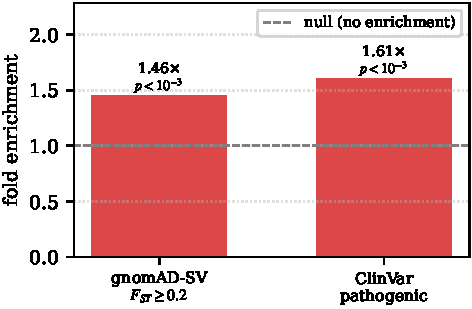
\includegraphics[width=\linewidth]{figs/fig_biology.pdf}
  \caption{\textsc{G2G} delta alleles on real AFR vs.\ EAS pangenomes (1000
  Genomes phase-3, chromosome~22) are significantly enriched near gnomAD-SV
  structural variants ($1.46\times$) and ClinVar pathogenic sites ($1.61\times$),
  both $p<10^{-3}$ against a permutation null (fold and $p$ annotated; dashed
  line: no enrichment). Synthetic positive/negative controls validate the
  statistic.}
  \label{fig:biology}
\end{figure}

\begin{figure}[t]
  \centering
  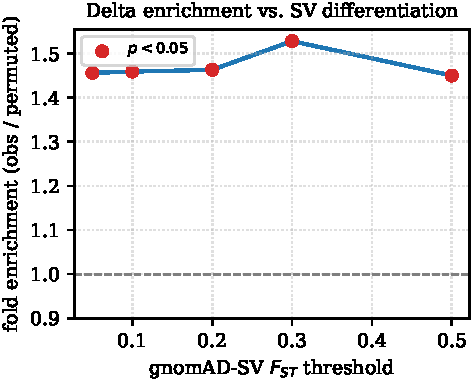
\includegraphics[width=\linewidth]{figs/fig_fst_sweep.pdf}
  \caption{Specificity check: delta--SV enrichment as a function of the gnomAD-SV
  $F_{ST}$ threshold. The fold is flat ($1.45$--$1.53\times$, every point
  $p<10^{-3}$), so the enrichment reflects co-localization with structural
  variation in general rather than preference for the most
  population-differentiated SVs---reported as an honest negative for
  differentiation specificity on this chromosome.}
  \label{fig:fstsweep}
\end{figure}
\section{Discussion}
\label{sec:discussion}

Every major decision in G2G traces to a measured property of the workload. Snarl-tree factorisation is what makes the problem practical: it decomposes the alignment into independent per-snarl subproblems, each solved optimally by LAPJV, though the snarl pairing itself remains a greedy heuristic. LAPJV replaces brute force because matching cost explodes with $k$ (Finding~1); centralised priority dispatch replaces static partitioning because per-snarl work is heavy-tailed (Finding~2), an argument the static-partition ablation confirms directly (Table \ref{tab:ablation}); and per-snarl struct packing plus flat sequence storage address the memory wall (Finding~3); the vEB inter-snarl ordering targets the same finding but is unexercised on depth-1 trees (\S\ref{sec:veb}). Two stages were originally quadratic: anchor detection and snarl decomposition. The minimiser index removes the first; the windowed sink search of \S\ref{sec:algo} makes the second linear for small snarls, though large-span SV snarls still fall back to the $O(|V|)$ search---the measured $N^{1.00}$ decomposition exponent (Fig.~\ref{fig:refdiffscaling}) reflects the short-variant-dominated test data, not the algorithm's worst case, and would rise on SV-rich inputs where the window overflows routinely.

\subsection{Described-general, evaluated-special}
\label{sec:gap}
The system as described is a nested-snarl, parallel, multi-representation engine. The system as evaluated operates on a strict special case: depth-1 snarl trees, short-variant-dominated synthetic graphs, and self-consistent coordinate representations. Table~\ref{tab:gap} makes the mismatch explicit.

\begin{table}[t]
  \centering
  \caption{Features described vs.\ features exercised in the evaluation. Every row where the evaluation column differs from the description column is a gap: the mechanism is implemented but untested under conditions where it can act.}
  \label{tab:gap}
  \footnotesize
  \begin{tabular}{lll}
    \toprule
    feature & described & evaluated \\
    \midrule
    snarl-tree depth & nested (arbitrary) & depth-1 only \\
    vEB layout & $O(N/B)$ on nested trees & degenerate ($\equiv$ BFS) \\
    nested recurrence & bottom-up DP & never fires \\
    decomposition & windowed + quadratic fallback & window never overflows \\
    variant representation & arbitrary & self-consistent only \\
    scheduler & LPT on heavy-tailed work & $67\%$ trivial $k{=}2$ tasks \\
    \bottomrule
  \end{tabular}
\end{table}

The individual caveats appear where the numbers are reported (Q1 scale gap, Q3 vEB tautology, \S\ref{sec:veb} depth-1 degeneracy, \S\ref{sec:algo} decomposition circularity), but the structural pattern deserves a unified statement: \emph{the quantitative evidence in this paper validates the system only in the special case}. The general-case mechanisms (nested recurrence, vEB locality, quadratic-fallback decomposition) are implemented—they compile, pass unit tests, and are togglable for ablation—but no experiment exercises them under conditions where they can engage. We report them as design provisions for the intended deployment target (Minigraph-Cactus graphs with nested snarls, SV-containing long-read panels, mixed-provenance inputs), not as validated contributions. The numbers that appear beside them ($1.01\times$, $N^{1.00}$) are measured where the mechanisms cannot act and should be read as confirming inertness, not benefit.

\subsection{Limitations}
The decomposer is DAG-only: although an optional vg-snarl backend can supply snarl boundaries, the allele enumeration and DP assume acyclicity, so tandem repeats (cycles) are out of scope and full cyclic support is future work. Snarl pairing is greedy rather than globally optimal: anchors mitigate this but a full tree-matching pairing is future work. The validation--deployment scale gap (\S\ref{sec:eval}, Q1) is the most pressing open risk: accuracy is measured at 5--50 snarls while deployment targets $10^6$--$10^7$, and the only at-scale check (parallel$=$sequential) is blind to scale-dependent errors. Closing this gap requires either a genome-scale ground truth or targeted stress tests for the identified failure modes (hash collisions, window overflow, greedy drift). G2G is single-machine; the $K>2$ multi-graph alignment problem and a distributed engine are natural extensions, as is GPU acceleration of the per-snarl matching, which is embarrassingly parallel across snarls.
\section{Conclusion}
\label{sec:conclusion}

We presented PanG2G, the first system that computes base-pair-resolution graph-to-graph alignments of pangenome variation graphs. The reference-anchored diff, the primary validated result, is single-threaded and exact under identical variant representation. It scales near-linearly to an 8-Gbp pair on one core at 100\% precision/recall on planted variants. A parallel snarl-pairing aligner is designed for the general case with the full systems specification: minimizer index, LAPJV matching, priority-dispatch scheduler and vEB layout. This is validated on small-scale depth-1 workloads ($50.1\times$ at 64 cores, $12.7\times$ vs.\ linearize-and-map at $h{=}200$). A biological run confirms the pipeline produces a delta on real data. This shows that graph-to-graph alignment is a viable pangenome-era primitive: the reference-anchored diff demonstrates it concretely, the parallel engine takes a first step toward the general case.

\paragraph{Availability.}
The PanG2G source code, the Python reference prototype, the synthetic graph generators (with the seeds used here), the experiment harnesses and the plotting scripts are available at \url{https://github.com/ahmadshakleya/G2G}. All real inputs are public: the 1000 Genomes phase-3 panel, GRCh38, gnomAD-SV \cite{collins2017svfst} and ClinVar \cite{landrum2018clinvar}; the repository includes scripts that download them and rerun every experiment and figure reported here.
% TODO: add Zenodo DOI of the archived release here once minted.

\bibliographystyle{IEEEtran}
\bibliography{refs.bib}

\end{document}